%
% Complete documentation on the extended LaTeX markup used for Insight
% documentation is available in ``Documenting Insight'', which is part
% of the standard documentation for Insight.  It may be found online
% at:
%
%     http://www.itk.org/

\documentclass{InsightArticle}

\usepackage[dvips]{graphicx}



%%%%%%%%%%%%%%%%%%%%%%%%%%%%%%%%%%%%%%%%%%%%%%%%%%%%%%%%%%%%%%%%%%
%
%  hyperref should be the last package to be loaded.
%
%%%%%%%%%%%%%%%%%%%%%%%%%%%%%%%%%%%%%%%%%%%%%%%%%%%%%%%%%%%%%%%%%%
\usepackage[dvips,
bookmarks,
bookmarksopen,
backref,
colorlinks,linkcolor={blue},citecolor={blue},urlcolor={blue},
]{hyperref}

\usepackage{url}


%  This is a template for Papers to the Insight Journal. 
%  It is comparable to a technical report format.

% The title should be descriptive enough for people to be able to find
% the relevant document.
\title{CTest Integration of Sikuli Automated GUI Testing}

% 
% NOTE: This is the last number of the "handle" URL that 
% The Insight Journal assigns to your paper as part of the
% submission process. Please replace the number "1338" with
% the actual handle number that you get assigned.
%
\newcommand{\IJhandlerIDnumber}{3196}

% Increment the release number whenever significant changes are made.
% The author and/or editor can define 'significant' however they like.
\release{0.00}

% At minimum, give your name and an email address.  You can include a
% snail-mail address if you like.
\author{Evan Schwab, Lydie Souhait, Nicolas Rannou, Kishore Mosaliganti\\
Arnaud Gelas, Sean Megason}
\authoraddress{Harvard Medical School, Megason lab}

\begin{document}

% Add hyperlink to the web location and license of the paper.
\IJhandlefooter{\IJhandlerIDnumber}


\ifpdf
\else
   %
   % Commands for including Graphics when using latex
   %
   \DeclareGraphicsExtensions{.eps,.jpg,.gif,.tiff,.bmp,.png}
   \DeclareGraphicsRule{.jpg}{eps}{.jpg.bb}{`convert #1 eps:-}
   \DeclareGraphicsRule{.gif}{eps}{.gif.bb}{`convert #1 eps:-}
   \DeclareGraphicsRule{.tiff}{eps}{.tiff.bb}{`convert #1 eps:-}
   \DeclareGraphicsRule{.bmp}{eps}{.bmp.bb}{`convert #1 eps:-}
   \DeclareGraphicsRule{.png}{eps}{.png.bb}{`convert #1 eps:-}
\fi

\maketitle

\ifhtml
\chapter*{Front Matter\label{front}}
\fi

\begin{abstract}
\noindent
\end{abstract}

\IJhandlenote{\IJhandlerIDnumber}

\tableofcontents
% ------------------------------------------------------------------------
\section{Introduction}

% ------------------------------------------------------------------------
\section{Sikuli}

% Feel free to change section titles
\subsection{What is sikuli?}

Sikuli~\cite{Sikuli:Documentation,Sikuli:Website,Yeh:2009:Sikuli} is a visual
technology to automate and test graphical user interfaces (GUI) using images
(screenshots). Sikuli includes \emph{Sikuli Script} and \emph{Sikuli IDE}.\\

\emph{Sikuli Script} automates anything you see on the screen without internal
API's support. Sikuli Script is a programming language that uses screen shot
images as variables and objects in order to automate graphical user interface
functions. The Sikuli Script is built on a Jython (Python for Java platform)
library which uses Python syntax in addition to a number of special Sikuli
functions for acquiring and handling screen shot images and performing mouse,
keyboard actions.\\

In the \emph{Sikuli IDE}, the user can write scripts that include screen shot
thumbnails so they can visually track the functions of their code. The most
useful functions from Sikuli scripts are conveniently found as
buttons on the IDE. When using the IDE, Sikuli then saves a script in a
directory with a unique extension .sikuli. The directory consists of a python
script file (script file to be used by sikuli), an html file, and a list of all
the screenshot images used in the script.


\subsection{Simple Sikuli example} % not related to gofigure...

Figure 1 shows the Sikuli-IDE for version 0.10.2.  On the left-hand side menu is a list
of commonly used Sikuli commands like  \emph{find}(),  \emph{click}(), and  \emph{type}().  The picture of
the camera within the parentheses indicates the screenshot input variable.  Clicking
on any of these menu functions will automatically set up the Sikuli screen shot mode, whereby
the Sikuli-IDE disappears and what is on the screen at that moment is available to capture 
by selecting a rectangular region of interest.  The function will then appear in the scripting domain
with the snap shot in parentheses as shown in Figure 1.  The user may also type in the function
and invoke the screen shot mode by clicking on the camera in the top menu or by using a
keyboard shortcut. The simple Sikuli script example in Figure 1 will open gedit Text Editor, type a message,
and save the file. (see Figure~\ref{fig:SimpleExample}).

\begin{figure}[htbp]
 \centering
 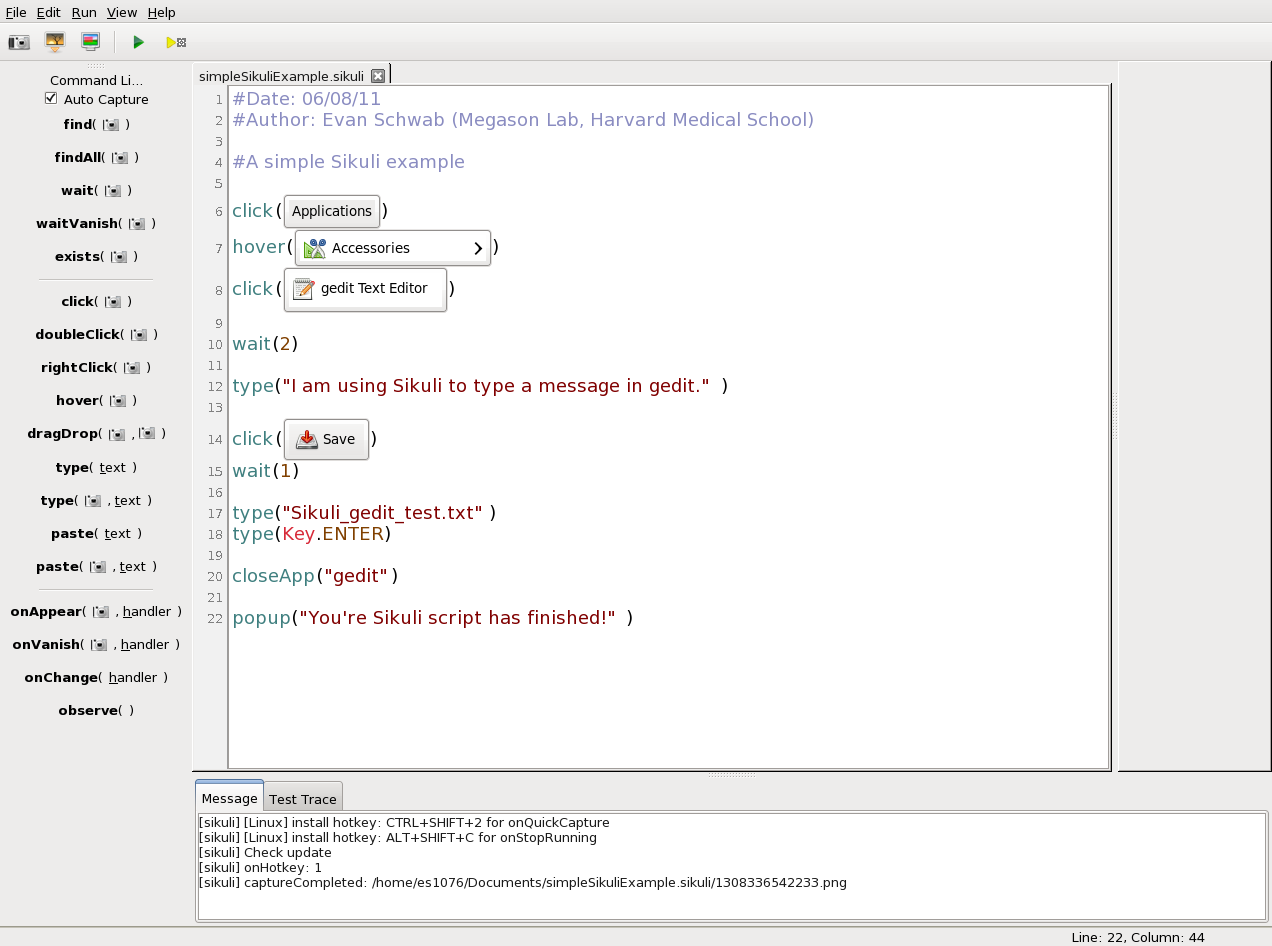
\includegraphics[width=0.99\textwidth]{Images/SimpleSikuliExample.png}
 % SimpleSikuliExample.png: 1280x1024 pixel, 72dpi, 45.16x36.12 cm, bb=0 0 1280 1024
 \caption{Simple Sikuli Script Example in Sikuli-IDE}
 \label{fig:SimpleExample}
\end{figure}

% ------------------------------------------------------------------------
\section{Integration with CTest}

% I'll write it this part
One of Sikuli's primary uses is the automation of GUI testing for software
developers. For GUI testing, it is useful to compartmentalize different software
functions and test each unit individually.\\

The newest versions of Sikuli come equipped with a Unit Testing feature based
on JUnit~\cite{}. Unit Testing can be called using the IDE or by command
line and enables the user to write multiple functions in a script which are
run individually. At the end of the run, the Sikuli output will tell the user
how many tests ran successfully and which ones failed and where.\\

Here we connect this Unit Testing feature to CTest, this allows us to report
results on public dashboard using CDash.


% ------------------------------------------------------------------------
\section{Example}

The Sikuli script in Figure 2 shows a fragment of a unit test for the GoFigure2 software.  The unit being tested here
is the Toolbar menu which consists of different modes used to analyze data set plots.
In total there are four modes which are represented in the first line as the vector Toolbar and for each
of these modes we want to test their expected mouse functions.  For instance, if we are in the zoom Toolbar mode
then we want the data set plot to zoom in when the user scrolls the mouse wheel forward.  Likewise,
if we are in pan mode then we want the plot to move to the left if the user holds down the left mouse button and moves
the mouse to the left.  Also importantly, we want to see that these two mouse actions are unique for their respective Toolbar modes;
the test will include an assertion that scrolling forward will zoom in when using zoom mode and will do nothing when using pan mode.\\

This breakdown of modes and actions lends itself to a nested for-loop scripting approach. By representing
these variables as a vector the software developers can easily add new modes or actions to each list to be tested, when
the software is updated. Similarly, the tester can easily replace any of the screenshot images with images of updated
GUI icons.\\  

In addition to representing the modes and actions
as the vectors Toolbar and Mouse, respectively, we've included the different data set plots in the vector ViewRegion.  
These images represent the  \emph{xy-},  \emph{xz-},  \emph{yz-}, and  \emph{xyz-}views of zebrafish microscopy data taken in the Megason Lab.  After capturing
these images we can then use them to locate their initial pixel coordinates within the GoFigure2 GUI using the \emph{find}() function.  These points become 
our reference positions to calculate directional movement.  For example, when testing the pan mode, we mark the initial position of each image,
use the \emph{mouseMove}() function to a chosen location, and then use \emph{find}() to obtain the new coordinates.  We can then assert if the image panned as it should have.
Similarly for zoom, we can first find the area of the image and then find the area of the zoomed in image.  To test the result when the user clicks 
in a certain mode, we've made use of Sikuli's \emph{assert exists}() function to ascertain the existence of our
desired results   (see Figure~\ref{fig:Gofigure2Example}).\\

This one GUI test is then combined with other GoFigure2 tests in succession and the Sikuli Unit Testing CTest integration will identify
which tests pass and which fail and when. Many of the units need to be tested in a certain order.  For example, in order to test the Toolbar modes
on the data sets, one first needs to test the software's data import functionality.

\begin{figure}[htp]
 \centering
 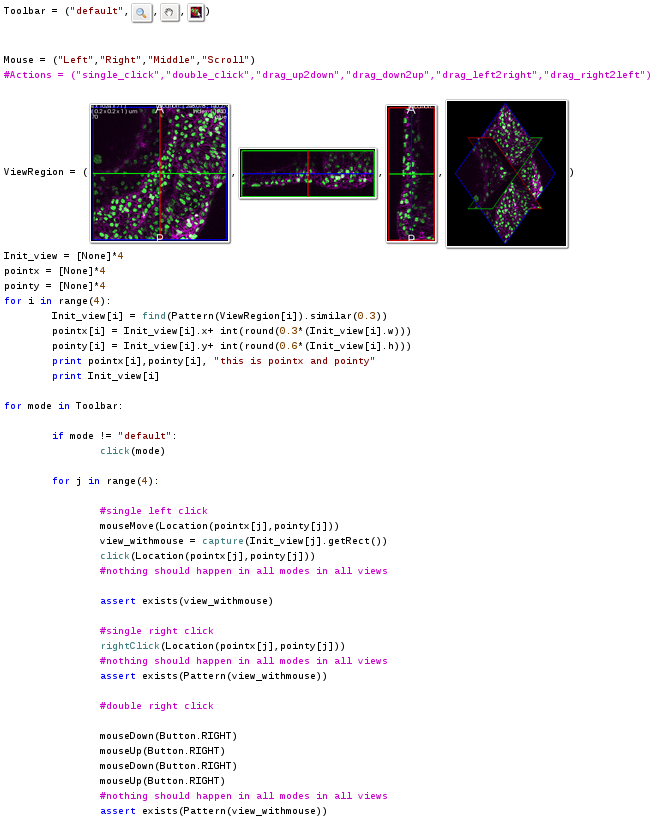
\includegraphics[width=0.99\textwidth]{Images/Gofigure2Example.png}
 % Gofigure2Example.png: 667x826 pixel, 72dpi, 23.53x29.14 cm, bb=0 0 667 826
 \caption{Sikuli Script for Gofigure2 GUI Testing}
 \label{fig:Gofigure2Example}
\end{figure}
% ------------------------------------------------------------------------
\section{Conclusion}

\clearpage

\bibliographystyle{plain}
\bibliography{InsightJournal,biblio}


\end{document}

